\chapter{Learning from Data}
\label{chapter:learningFromData}

The following exercises are logic-based, combinatorial puzzles. The idea is that pupils need to conclude the solution by a partially completed grid.

\section{Row of Trees}
\label{section:treeRow}

\subsection{Concept}
The row of trees is a one dimensional grid i.e a row either of size 3 or 4. In every row there is exactly one tree of every height between 1 and 3 (Fig. \ref{fig:trees_3}) or 4 (Fig. \ref{fig:trees_4}) respectively. At both ends of the row the amount of tree visible from this end of the row is given.
Pupils are given an empty row with only the number of trees seen from both ends of the row and need to place a tree of each height such the aforementioned rules are met.

\begin{figure} 
    \centering
    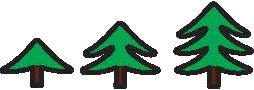
\includegraphics[width=0.4 \columnwidth]{figures/trees_3.png}
    \caption{Trees from height 1 to 3} 
    \label{fig:trees_3} 
\end{figure}

\begin{figure} 
    \centering
    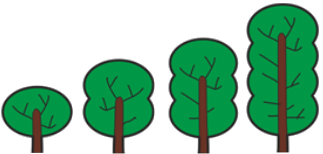
\includegraphics[width=0.4 \columnwidth]{figures/trees_4.png}
    \caption{Trees from height 1 to 4} 
    \label{fig:trees_4} 
\end{figure}

\begin{example}
    For a row of size 3, if given the value 2 for both ends of the row, then one possible solution to the puzzle is shown in figure \ref{fig:tree_row_example}.
\end{example}

\begin{figure} 
    \centering
    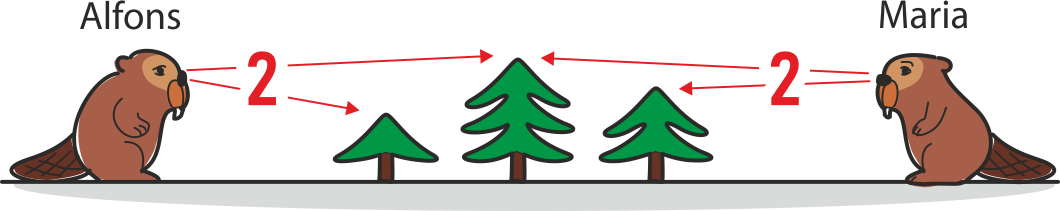
\includegraphics[width=0.8 \columnwidth]{figures/tree_row_example.png}
    \caption{Visualization of the puzzle solution from the tree row example} 
    \label{fig:tree_row_example} 
\end{figure}

\subsection{Implementation}

\section{Tree Sudoku}
\label{section:treeSudoku}

\subsection{Concept}
Tree sudoku is similar to the well known traditional sudoko with the difference that trees of different heights are placed instead of numbers, and for end of every row and collumn the number of visible trees is given. Otherwise, the puzzle follows the same rules as the row of trees and is either of size 3x3 or 4x4.

\begin{example}
    An example of a 3x3 tree sudoku is shown in figure \ref{fig:tree_sudoku_example}
\end{example}

\begin{figure} 
    \centering
    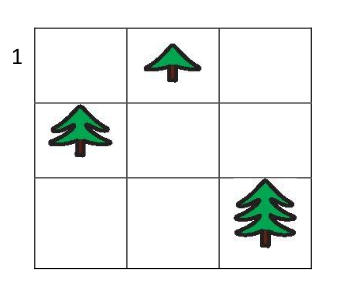
\includegraphics[width=0.4 \columnwidth]{figures/tree_sudoku_example.png}
    \caption{Example of an unsolved 3x3 tree sudoku} 
    \label{fig:tree_sudoku_example} 
\end{figure}
% https://www.bowdoin.edu/~sbarker/teaching/courses/ds/18fall/files/lab4.pdf

\subsection{Implementation}
% sudoku solver